\chapter{Quantum Machine Learning}

Quantum Machine Learning (QML) explores the interplay of ideas from quantum computing and
machine learning~\cite{Biamonte_2017}.
For example, QML investigates whether quantum computers can speed up the time it takes
to train or evaluate a machine learning model. On the other hand, the QML community
leverages techniques from machine learning to devise new quantum error-correcting codes~\cite{Roffe_2019}, 
estimate the properties of quantum systems, or develop new quantum algorithms.\\
As previously stated, QML is the intersection of Machine Learning and Quantum Computing and this intersection can be 
factorised in four main areas:


\begin{itemize}
    \item \textbf{Classical for Classical (CC)}.\\ This area actually do not have a quantum component and 
    it indicates those purely classical cases when a classical machine learning algorithm is used to solve 
    a classical task.
    \item \textbf{Classical for Quantum (CQ)}.\\ This area indicates those studies which aim to use classical
    machine learning procedures to deal with problems in the quantum physics domain.
    \item \textbf{Quantum for Classical (QC)}.\\ This area instead refers to using quantum resources or algorithms, 
    for example variational quantum algorithms, to analyse or process classical information, 
    that is data that come from a classical source.
    \item \textbf{Quantum for Quantum (QQ)}.\\ This last area is arguably the most compelling yet unexplored
    application of Quantum Machine Learning, regarding the use of quantum processors to
    learn or study properties of quantum systems.
\end{itemize}

In my Master's thesis I have focused only on the \textit{Quantum for Classical} area.\\


\section{Linear quantum models: explicit models, implicit models, data re-uploading models}

In the following sections we will compare and discuss three different quantum models: \textit{explicit quantum models}; 
\textit{quantum kernel models} (implicit quantum models); \textit{data re-uploading circuits} 
(figure \ref{fig:quantum-models}).\\
In explicit models the encoded data point is measured according to a variational observable that specifies its label.
In implicit quantum models, the weighted inner products of encoded datapoints are used to assign labels
Since data re-uploading models have an alternation of data-encoding and variational unitaries, they 
can be seen as a generalization of explicit models.


\begin{figure}[h]
    \centering
    \includegraphics[scale=0.7]{sections/chapters/Quantum-Machine-Learning/Images/quantum-models.pdf}
    \caption{This figure is taken directly from \cite{Jerbi_2023}. This figures shows three different quantum models:
    (a) an explicit quantum model; (b) a quantum kernel model; (c) a data re-uploading circuit.}
    \label{fig:quantum-models}
\end{figure}

First of all, let's discuss how explicit and implicit models can both be described as linear quantum models and then
we will highlight their differences.\\
A quantum machine learning model deals with data, thus the first step is to upload the data of the 
problem into the model.
Data can be either \textit{classical} $\{\bm{x}_i\}_{i=1}^m \in \chi \subseteq \mathbb{R}$ 
or \textit{quantum}, such as a set of states $\{ |\psi_i\rangle \}_{i=1}^m \in \mathcal{H} = C^{2n}$, 
where $\mathcal{H}$ is the Hilbert space of a quantum system of n qubits.\\
Let's discuss separately how to upload classical and quantum data on a quantum computer.

\begin{enumerate}
    \item Classical data.\\
    The procedure that uploads classical data $\{\bm{x}_i\}_{i=1}^m$ on a quantum computer is called
    \textit{feature embedding}.
    Specifically, this is achieved by a unitary $U(\bm{x})$ which depends on the data:

    \begin{align}
        \phi : \chi &\rightarrow \mathcal{F} = \mathcal{H}\\
        \bm{x} &\mapsto |\phi(\bm{x})\rangle = U_{\phi}(\bm{x}) |0\rangle^{\otimes n}\\
    \end{align}

    where $\mathcal{F}$ is the feature space, which in this case is the Hilbert space $\mathcal{H}$ of 
    $2^n \times 2^n$ hermitian operators.
    We have numerous different feature embedding maps $U(\bm{x})$: \textit{angle encoding}, \textit{amplitude encoding},
    \textit{Qsample encoding}.\\
    For example the angle encoding consists in a different Pauli rotation for each component of the datapoint
    (thus requiring one qubit per dimension of the input data $d = n$):

    \begin{align}
        U(\bm{x}) = \otimes_{i=1}^n R_{P_i}(x_i) 
        \qquad 
        \bm{x} = (x_1, x_2, ..., x_N), P_i = {X, Y, Z}
    \end{align}

    In the amplitude encoding each component of a datapoint of dimension d becomes the amplitude of a vector 
    of the computational basis, thus requiring a number of qubit $n = \left\lceil log_2(d) \right\rceil$
    \footnote[1]{
        The amplitude encoding requires that the components of each datapoint $\bm{x}$ must be normalized. 
        This a fundamental restriction because 
        this means that quantum states represent the data one less dimension or with one less degree of freedom.
        For example a classical two dimensional vector $(x_1, x_2)$ can only be associated with an amplitude 
        vector $(\alpha_1, \alpha_2)$ of a qubit which fulfils $|\alpha_1|^2 + |\alpha_2|^2 = 1$.
    }.

    \begin{align}
    \bm{x} = \begin{pmatrix}
        x_1 \\
        x_2 \\
        ... \\
        x_{2^n} \\
    \end{pmatrix}
    \qquad
    \rightarrow
    \qquad
    \psi = \sum_i^{2^n} x_j | j \rangle
    \end{align}

    \item Quantum data.\\
    If we want to upload a certain quantum state $|\psi_i\rangle$ on a quantum computer, we have to determine
    the appropriate unitary $U_i$, which applied to the ground state gives $|\psi_i\rangle$:
    
    \begin{equation}
        U_i |0\rangle^{\otimes n} = |\psi_i\rangle
    \end{equation}
\end{enumerate}

After we have embedded our data on a quantum computer, a linear function in the quantum feature space 
$\mathcal{F}$ is defined by:

\begin{equation}
    f(\bm{x}) = Tr[\rho(\bm{x})O]
\end{equation}

for some hermitian observable $O \in \mathcal{F}$.\\
Explicit and implicit models differ in the way they define the family of observable 
$\{ O \}$ they each consider.

\subsection{Explicit models}

An explicit quantum model using the feature encoding $U_{\phi}(\bm{x})$ is defined by a variational 
family of unitaries $V(\bm{\theta})$ and a fixed observable O:

\begin{equation}
    f_{\bm{\theta}}(\bm{x}) = Tr[\rho(\bm{x})O_{\bm{\theta}}]
\end{equation}

for $O_{\bm{\theta}} = V(\bm{\theta})^{\dagger} O V(\bm{\theta})$

\subsection{Implicit models}

Implicit models are defined by the datapoints $\{ \bm{x}^{(1)}, \bm{x}^{(2)}, ..., \bm{x}^{(M)} \}$ of a given training set
$\mathcal{D}$ and in particular they are a linear combination of the innerproducts of encoded datapoints:

\begin{equation}
    f_{\bm{\alpha}, \mathcal{D}}(\bm{x}) = \sum_{i=1}^M \alpha_m k(\bm{x}, \bm{x}^{(m)}) = Tr[\rho(\bm{x}), \rho(\bm{x}^{(m)})]
\end{equation}

By the linearity of the trace we can express any implicit model as a linear model in $\mathcal{F}$, defined by the 
observable:

\begin{equation}
    O_{\bm{\alpha}, \mathcal{D}} = \sum_{i=1}^M \alpha_m \rho(\bm{x}^{(m)})
\end{equation}


\subsection{Data re-uploading models}

\cite{P_rez_Salinas_2020} introduced the \textit{re-uploading} encoding technique,
drawing inspiration from classical neural networks.
The key idea that inspired Salinas et al is that a feed-forward neural network processes data several times
(in each layer), one for each neuron in the considered hidden layer. 
Therefore, strictly speaking, data is \textit{re-uploaded} multiple times onto the neural network.
This key concept is illustrated in figure \ref{fig:data-reuploading-diagram}.



% \subcaption[⟨list entry⟩]{⟨heading⟩}[⟨width⟩][⟨inner-pos⟩]{⟨contents⟩}
% list entry: nome interno che verrà usato se generata la lista delle figure.
% heading: subcaption
% width: larghezza del parbox creato
% inner-pos: posizione che avrà l'immagine nel parbox
% contents: immagine
\begin{figure}[h]
    \centering
    \begin{subfigure}[b][.45\textwidth]
        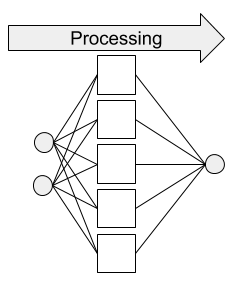
\includegraphics[width=0.25\textwidth]{sections/chapters/Quantum-Machine-Learning/Images/Neural_network.png}
    \end{subfigure}
    \begin{subfigure}[b][.45\textwidth]
        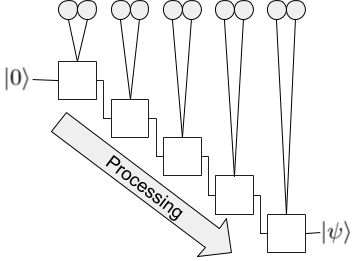
\includegraphics[width=0.5\textwidth]{sections/chapters/Quantum-Machine-Learning/Images/Quantum_scheme.png}
    \end{subfigure}
    \caption{
        Schemes of a one layer neural network and a single-qubit quantum circuit with data re-uploading.
        In the neural network the data is uploaded in each neuron of the hidden layer, hence data is 
        \textit{re-uploaded} multiple times.
        In a similar way the data is introduced classically numerous times in the circuit.
        The key difference between the two architectures is that each neuron of a neural network processes the 
        data in parallel and simultaneously, whereas the single-qubit quantum circuit with data re-uploading 
        processes the data sequentially.}
    \label{fig:data-reuploading-diagram}
\end{figure}

In a single-qubit quantum circuit with data re-uploading, data is introduced as a rotation of the qubit.
Since every unitary can be expressed as the product of three rotation gates, we can define the angles as a linear
combination of weights and coordinates of the data\footnote[1]{Just like in a neuron of neural network.}.

\begin{equation}
    U(\bm{\phi}) = R_Z(\phi_1) R_Y(\phi_2) R_Z(\phi_3)
\label{}
\end{equation}

For instance, if data is 3-dimensional $\bm{x} = (x_1, x_2, x_3)$:

\begin{align}
    \phi_1 &= x_1 \cdot w_1 + b_1 \\
    \phi_2 &= x_2 \cdot w_2 + b_2 \\
    \phi_3 &= x_3 \cdot w_3 + b_3 \\
\end{align}

If data has a dimension greater than 3, we will need more than one unitary to encode a datapoint.
In general, if data has dimension \textit{d} we will need \(\left\lfloor \frac{d}{3} \right\rceil\) unitaries.
Each repetition of this \(\left\lfloor \frac{d}{3} \right\rceil\) unitaries to encode the data constitutes 
one layer of the architectures.

\begin{figure}
    \centering
    \begin{quantikz}
        \lstick{$\ket{0}$} &&& \gate{U(\phi_1, x)} 
        \gategroup[1,steps=1, style={dashed,rounded corners,fill=blue!20,inner xsep=6pt}, background, label style={label
        position=below, yshift=-0.4cm}]{L(1)} 
        &&& \ \ldots \ &&& \gate{U(\phi_N, x)} 
        \gategroup[1,steps=1, style={dashed,rounded corners,fill=blue!20,inner xsep=6pt}, background, label style={label
        position=below, yshift=-0.4cm}]{L(N)}
        &&& \meter{}
    \end{quantikz}
    \caption{The quantum circuit of a data re-uploading model is divided into layers L(i), which constitutes 
    the building blocks of this architecture.}
\end{figure}

Figure


\begin{figure}[h]
    \centering
    \begin{subfigure}[b][0.45\textwidth]
        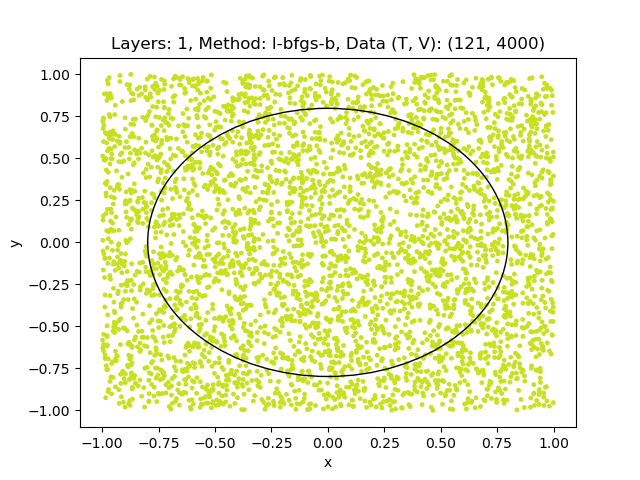
\includegraphics[width=\textwidth]{sections/chapters/Quantum-Machine-Learning/Images/Data-Re-Uploading/Layer1-A.png}
    \end{subfigure}
    \begin{subfigure}[b][0.45\textwidth]
        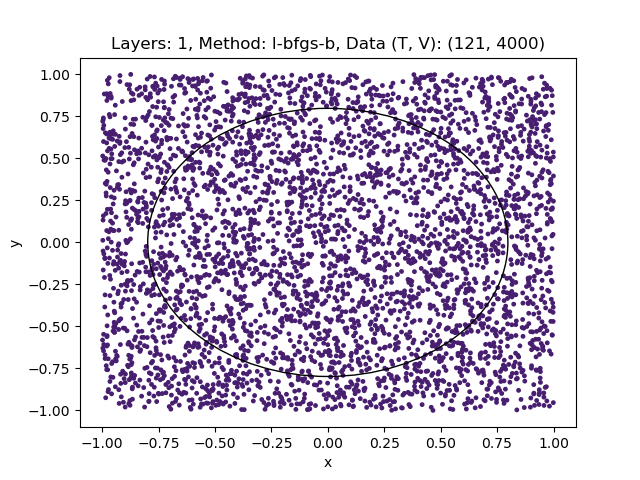
\includegraphics[width=\textwidth]{sections/chapters/Quantum-Machine-Learning/Images/Data-Re-Uploading/Layer1-B.png}
    \end{subfigure}
    \begin{subfigure}[b][0.45\textwidth]
        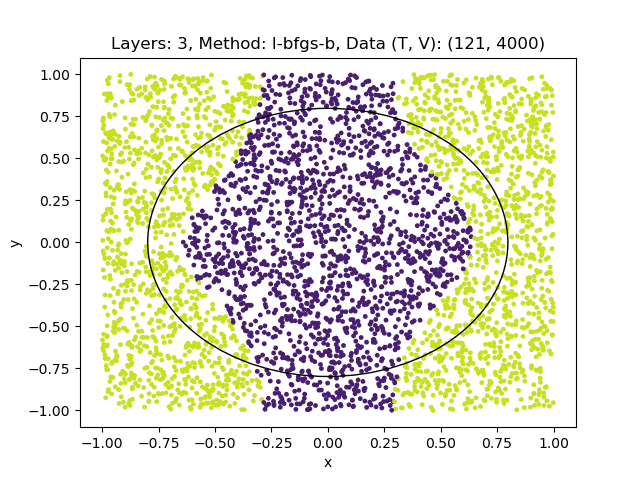
\includegraphics[width=\textwidth]{sections/chapters/Quantum-Machine-Learning/Images/Data-Re-Uploading/Layer3-A.png}
    \end{subfigure}
    \begin{subfigure}[b][0.45\textwidth]
        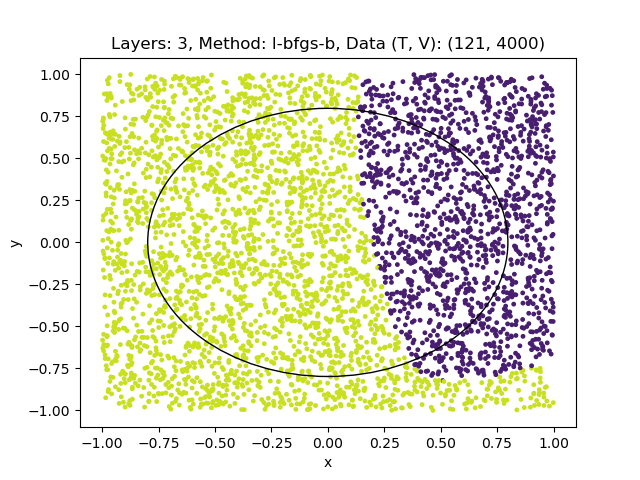
\includegraphics[width=\textwidth]{sections/chapters/Quantum-Machine-Learning/Images/Data-Re-Uploading/Layer3-B.png}
    \end{subfigure}
    \begin{subfigure}[b][0.45\textwidth]
        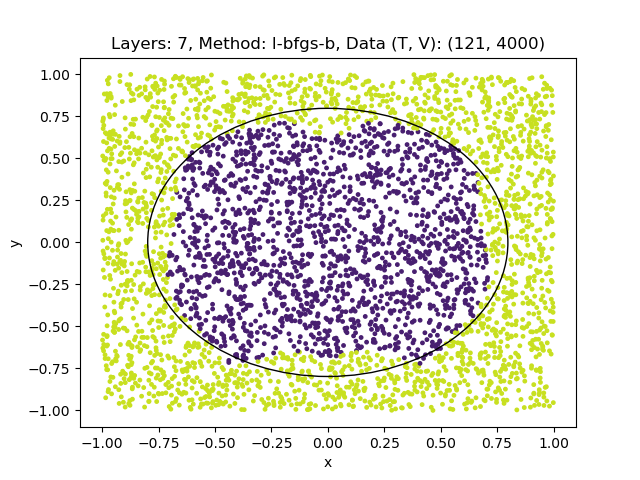
\includegraphics[width=\textwidth]{sections/chapters/Quantum-Machine-Learning/Images/Data-Re-Uploading/Layer7-A.png}
    \end{subfigure}
    \begin{subfigure}[b][0.45\textwidth]
        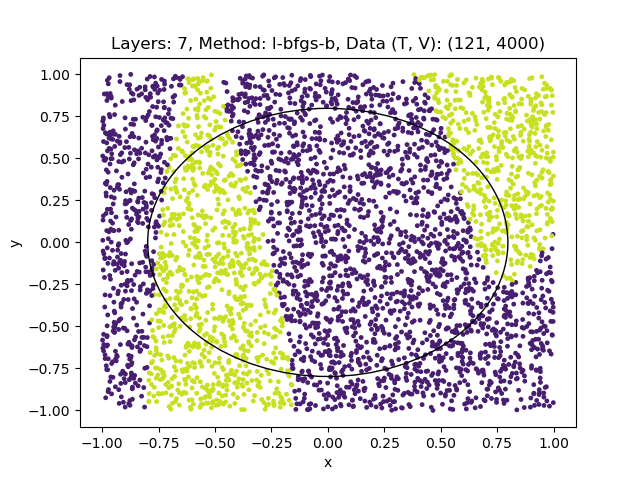
\includegraphics[width=\textwidth]{sections/chapters/Quantum-Machine-Learning/Images/Data-Re-Uploading/Layer7-B.png}
    \end{subfigure}
    \begin{subfigure}[b][0.45\textwidth]
        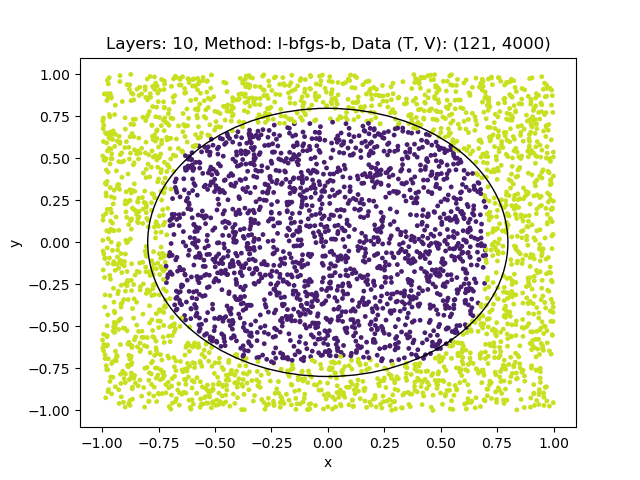
\includegraphics[width=\textwidth]{sections/chapters/Quantum-Machine-Learning/Images/Data-Re-Uploading/Layer10-A.png}
    \end{subfigure}
    \begin{subfigure}[b][0.45\textwidth]
        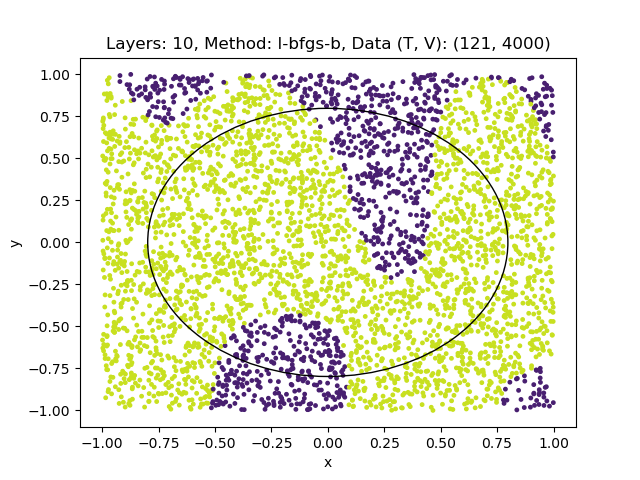
\includegraphics[width=\textwidth]{sections/chapters/Quantum-Machine-Learning/Images/Data-Re-Uploading/Layer10-B.png}
    \end{subfigure}
\end{figure}


\section{Variational Quantum Algorithms}

The state of the art of Quantum Machine Learning has as main highlight the development
of algorithms that have been proven to have a quantum advantage in computational
complexity over classical algorithms~\cite{Sweke_2021, Liu_2021, Jerbi_2021}.
However, these algorithms require a fault-tolerant quantum computer~\cite{shor}, which is able to
continuously correct errors that arise during computation, ensuring the stability and
reliability of the quantum processes over extended periods.
As we are still many years away from fault tolerant quantum computation, the QML
community has developed a great interest toward possible applications of current and
near-term quantum devices (NISQ devices)~\cite{Preskill_2018}, which are not capable of continuous
quantum error correction.
In particular, the QML research community has developed a new class of quantum
procedures called variational quantum algorithms (VQA)~\cite{Cerezo_2021} to take advantage of current
and near-term quantum hardware.\\
However no quantum advantage has been proven for this algorithms, yet.\\

A VQA is a \textit{hybrid quantum-classical} algorithm with different components:

\begin{enumerate}
    \item \textbf{Encoding block}.\\
    The first component is the encoding block, which is responsible to encode the data of the problem in the 
    algorithm.
    \item \textbf{Parametrized Quantum Circuit (PQC)}.\\
    The second component is a parametrized quantum circuit U($\theta$), which is a circuit made of numerous gates. The parameters are usually 
    the angles of the circuit and they can be tuned to enhance the algorithm's performance for completing a specific task. 
    \item \textbf{Decoding Block}.\\
    The third component is the decoding block, which consists in measuring the PQC.
    \item \textbf{Optimization}.\\
    The valuable information extracted when measuring the PQC is used to evaluate a objective function.
    This objective function is then optimized, and this procedure suggests improved candidates 
    for the parameters $\theta$, starting from random or pre-trained initial values.
\end{enumerate}

The crucial point to emphasize of a VQA is that the PQC can be executed on current quantum
devices, while the computational demanding task of optimizing the objective function is
performed by a classical computer, which is far more reliable then current NISQ devices.
Therefore, the trademark of VQAs is that they use a quantum computer to estimate the cost function (or its gradient) 
while leveraging the power of classical optimizers to train the parameters: this is why they are called
\textit{hybrid quantum-classical} algorithms.\\
Many different VQAs have been designed to tackle standard machine learning tasks, such
as classification, regression or optimization.
CITAZIONE

\subsection{Parametrized Quantum Circuit}


Parameterized Quantum Circuits are the core of every VQA.\\
Consequently, it is crucial to design circuits that are not only \textit{easy to train} but also capable of 
\textit{generalizing} from the training data and sufficiently \textit{expressive} to identify an optimal solution 
for the given task.\\

A PQC, also known as \textit{quantum neural network}, can be expressed as a series of L parametrized unitaries:

\begin{equation}
    U(\theta) = \prod_{i=1}^L U_i(\theta_i)
\label{Eq:definition-PQC}
\end{equation}

where $\theta = (\theta_1, ..., \theta_L)$ is a set of tunable parameters.
This parameters are updated by optimizing a loss function:

\begin{comment}
\[
    \ell_{\theta}(\rho, O) = \text{Tr}\left[\rho(\theta)O\right]
    \qquad
    \rightarrow
    \qquad
    \argmin_{\theta} l_{\theta}(\rho, O)
\]
\end{comment}


More general loss functions exist, but this case is already relevant.\\
The main properties of a PQC are \textit{expressivity}~\cite{hubregtsen2020, Sim_2019, Bravo_Prieto_2020, 
Wu_2021, Herman_2023, Haug_2021, Holmes_2022}, \textit{generalization}~\cite{Caro_2020, Abbas_2021, Banchi_2021,
Bu_2023, bu2021, Bu_2022, Du_2022, Peters_2023, Caro_2023} and \textit{trainability}~\cite{McClean_2018, 
Cerezo_2021, Arrasmith_2021, Kim_2021, Wang_2021, Pesah_2021, marrero2021, Larocca_2023}.

\paragraph{Trainability}

As in classical machine learning, variational quantum algorithms can suffer from the problem of vanishing 
gradient, or in QML terms \textit{Barren Plateaus} (BP).
A common definition of BP for VQAs is the following:

\begin{defn*}[Barren Plateaus]
    A VQA exhibits a BP if its loss function, or its gradients, concentrate exponentially about their mean 
    in the number of qubits n
    \footnote[1]{The two definitions of Barren Plateaus — one involving gradients and the other 
    involving the loss function — are not equivalent. The definition based on the loss function is 
    unambiguous, whereas the definition in terms of partial derivatives can be less clear. The ambiguity 
    arises because some partial derivatives might be exponentially concentrated while others are not. In such 
    cases, the loss function would not exhibit exponential concentration, indicating that the two definitions 
    are not equivalent. They become equivalent only when \textit{all} the gradients are exponentially concentrated 
    \cite{Arrasmith_2022}.}.
\end{defn*}

This means that, as the number of qubits n increases, the gradients of the loss function (or the loss function itself) 
tend to concentrate around an average value with increasing probability.    
The average value around which the gradient must concentrate in order to exhibit BP must be very 
small\footnote[1]{\cite{McClean_2018} demonstrated that, under broad conditions, random parameterized quantum 
circuits have an average gradient value of zero.}.
In fact, if the gradient were concentrated around a non-infinitesimal value, it would mean that the 
algorithm is still learning.
Intuitively, this means that the optimization landscape is mostly flat and featureless and
that slightly changing the model’s parameters $\theta$ results in only an exponentially small change in the loss
function value or its gradient.\\

The probabilistic nature of Quantum Mechanics forces us to measured a finite amount of times N the PQC to determine
the average value of an observable.
The statistical uncertainty related to the average value is inversely proportional to $\sqrt{N}$.
Therefore, if the loss function has an exponential concentration (which means that the changes of the loss function 
from one epoch to the following are exponentially suppressed), we need an exponential amount of shots to resolve this
changes, rendering the algorithm inefficient and non-scalable.
 

Two main types of BPs exist:

\begin{comment}
\begin{enumerate}
    \item \textbf{Probabilistic concentration and narrow gorges}.\\
    The most common type of BP is known as \textit{probabilistic concentration}.

    \begin{equation}
        Var_{\theta} \[ \ell_{\theta}(\rho, O) \] or Var_{\theta} \[ \partial_{\mu} \ell_{\theta}(\rho, O) \] \in \mathcal{O}(\frac{1}{b^n})
    \end{equation}

    where $b > 1$. Chebyshev's inequality implies for any $\delta > 0$:

    \begin{align}
        Pr(|\ell_{\theta}(\rho, O) - \mathbb{E}_{\theta}(\ell_{\theta}(\rho, O))| \ge \delta) \in \mathcal{O}(\frac{1}{b^n})\\
        Pr(|\partial_{\mu} \ell_{\theta}(\rho, O) - \mathbb{E}_{\theta}(\partial_{\mu} \ell_{\theta}(\rho, O))| \ge \delta) \in \mathcal{O}(\frac{1}{b^n})\\
    \end{align}

    which means that the probability that the loss deviates from its mean is exponentially small.\\
    Probabilistic BP imply a mostly flat landscape with some \textit{narrow gorge}.
    
    \item \textbf{Deterministic concentration}.\\
    A deterministic BP arises when $\forall \theta$:
    \begin{align}
        |\ell_{\theta}(\rho, O) - \mathbb{E}_{\theta}(\ell_{\theta}(\rho, O))| \in \mathcal{O}(\frac{1}{b^n})\\
        |\partial_{\mu} \ell_{\theta}(\rho, O) - \mathbb{E}_{\theta}(\partial_{\mu} \ell_{\theta}(\rho, O))| \in \mathcal{O}(\frac{1}{b^n})\\
    \end{align}

    where $b > 1$.
    Deterministic BP do not even admit narrow gorges.
\end{enumerate}
\end{comment}

A possible method to determine if the loss or the gradients are concentrating was introduced by \cite{McClean_2018}.
They randomly sampled parameters and computed how the variance scales with the number of qubits 
(figure \ref{figure:McClean}).
In particular, this paper showed that for a large class of random quantum circuits the average value of the gradient of the objective 
function is zero and the probability that any given instance of such a random circuit deviates from this average 
value by a small constant $\epsilon$ is exponentially small in the number of qubits.
The region where the average value of the gradient is zero does not correspond to a local minimum, but rather an 
exponentially large plateau in the landscape of the parameters.\\

\begin{figure}
    \centering
    \includegraphics[width=.45\textwidth]{sections/chapters/Quantum-Machine-Learning/Images/ProjectionGradientVar.pdf}
    \includegraphics[width=.45\textwidth]{sections/chapters/Quantum-Machine-Learning/Images/ProjectionGradientVarLayers.pdf}
    \caption{These are the original images from the paper by \cite{McClean_2018}. 
    The image on the left shows the variance of the gradient of a two-local Pauli term plotted as a function of 
    the number of qubits: an exponential decay is observed as a function of the number 
    of qubits for both the expected value and its spread.
    The image on the right shows the variance of the gradient of a two-local Pauli term plotted as a function of the 
    number of layers. The different lines correspond to all even numbers of qubits between 
    2 and 24, with 2 qubits being the top line, and the rest being ordered by qubit number. This shows 
    the convergence of the variance as a function of the number of layers to a fixed value determined by the 
    number of qubits.
    }
    \label{figure:McClean}
\end{figure}

Other possible quantities have introduced to study if a BP occurs: \textit{landscape's information content} \cite{P_rez_Salinas_2024}, 
\textit{local state's entanglement} \cite{Sack_2022}, \textit{landscape's Fourier coefficients} \cite{okumura2023, Nemkov_2023}.

The final remark on trainability is to discuss the origin of BPs:

\begin{itemize}
    \item \textbf{Curse of dimensionality}.\\
    \item \textbf{Circuit expressiveness}.\\
    \item 
\end{itemize}

\paragraph{Generalization}


\paragraph{Expressivity}



\section{Quantum Machine Learning}

\subsection{Linear quantum models: quantum classifiers and kernel methods}

\subsection{Data reuploading models and Quantum Neural Network}

\subsection{Deriving the Fourier expansion}

\subsection{A single-qubit data reuploading circuit}

\subsection{Quantum Neural Networks}

\subsection{Generalization of QML models}

\subsection{The power of quantum machine learning}







